% IJA Ukol c. 3
% Date: 2012-03-24
% Author: David Molnar (xmolna02)
% Email: xmolna02@stu.fit.vutbr.cz

\documentclass[12pt,a4paper,titlepage,final]{article}

% slovencina a fonty
\usepackage[slovak]{babel}
\usepackage[utf8]{inputenc}
% balicky pro odkazy
\usepackage[bookmarksopen,colorlinks,plainpages=false,urlcolor=blue,unicode]{hyperref}
\usepackage{url}
% obrazky
\usepackage{graphics}
\usepackage{epstopdf}
\usepackage[dvipdf]{graphicx}
% velikost stranky
\usepackage[top=3.5cm, left=2.5cm, text={17cm, 24cm}, ignorefoot]{geometry}

\begin{document}

%%%%%%%%%%%%%%%%%%%%%%%%%%%%%%%%%%%%%%%%%%%%%%%%%%%%%%%%%%%%%%%%%%%%%%%%%%%%%%
% titulna strana


\def\author{Dávid Molnár}
\def\email{xmolna02@stud.fit.vutbr.cz}
\def\projname{Návrh architektúry projektu IJA}

\begin{titlepage}

% \vspace*{1cm}
\begin{figure}[!h]
  \centering
  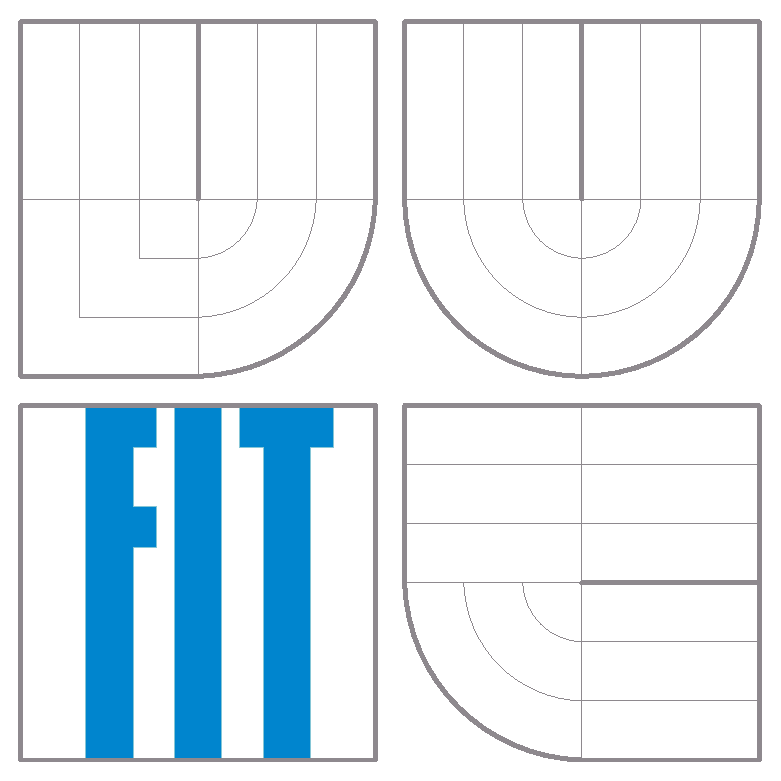
\includegraphics[height=5cm]{img/logo.eps}
\end{figure}

\vfill

\begin{center}
\begin{Large}
Dokumentácia k úkolu na predmet IJA\\
\end{Large}
\bigskip
\begin{Huge}
\projname\\
\end{Huge}
\begin{large}
úkol č. 3
\end{large}
\end{center}

\vfill

\begin{center}
\begin{Large}
\today
\end{Large}
\end{center}

\vfill

\begin{flushleft}
\begin{large}
\begin{tabular}{ll}
Autor: & \author, \url{\email} \\
 & Fakulta Informačních Technologií \\
 & Vysoké Učení Technické v~Brně \\
\end{tabular}
\end{large}
\end{flushleft}
\end{titlepage}


%%%%%%%%%%%%%%%%%%%%%%%%%%%%%%%%%%%%%%%%%%%%%%%%%%%%%%%%%%%%%%%%%%%%%%%%%%%%%%
% obsah
\pagestyle{plain}
\pagenumbering{roman}
\setcounter{page}{1}
%\tableofcontents

%%%%%%%%%%%%%%%%%%%%%%%%%%%%%%%%%%%%%%%%%%%%%%%%%%%%%%%%%%%%%%%%%%%%%%%%%%%%%%
% textova sprava
\newpage
\pagestyle{plain}
\pagenumbering{arabic}
\setcounter{page}{1}


%%%%%%%%%%%%%%%%%%%%%%%%%%%%%%%%%%%%%%%%%%%%%%%%%%%%%%%%%%%%%%%%%%%%%%%%%%%%%%
\section{Informácie o projektu a týmu} \label{tym}
%%%%%%%%%%%%%%%%%%%%%%%%%%%%%%%%%%%%%%%%%%%%%%%%%%%%%%%%%%%%%%%%%%%%%%%%%%%%%%
Projekt IJA je vytvorenie aplikáciu pre hru Dáma.

Tým je \textbf{jednočlenný}. Jediný člen som ja, Dávid Molnár (xmolna02).

%%%%%%%%%%%%%%%%%%%%%%%%%%%%%%%%%%%%%%%%%%%%%%%%%%%%%%%%%%%%%%%%%%%%%%%%%%%%%%
\section{Návrh architektúry projektu} \label{navrh}
%%%%%%%%%%%%%%%%%%%%%%%%%%%%%%%%%%%%%%%%%%%%%%%%%%%%%%%%%%%%%%%%%%%%%%%%%%%%%%

% aplikační třídy, rozhraní, balíky a jejich vazby

\begin{figure}[t]
  \centering
  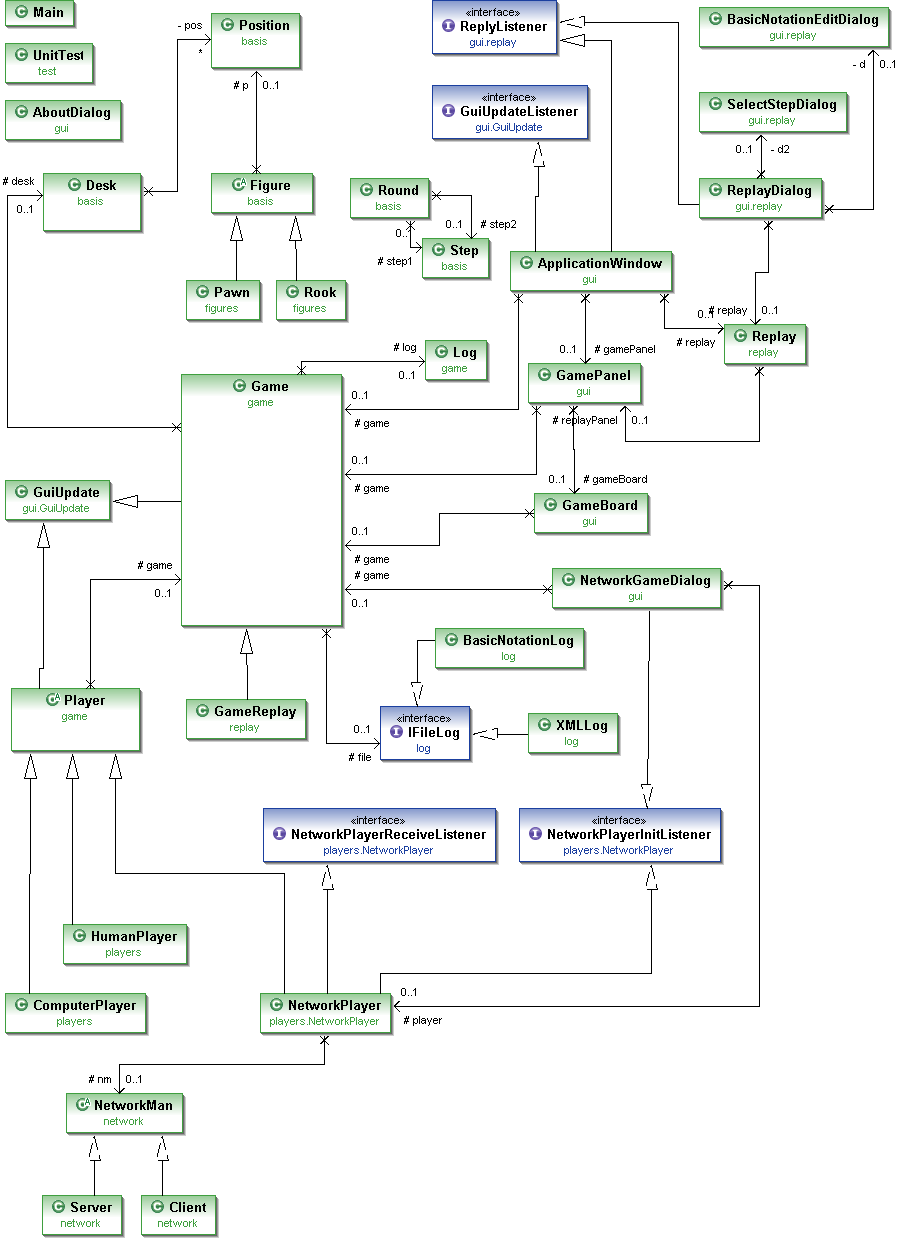
\includegraphics[height=23cm]{img/cd.png}
  \caption{Class diagram projektu}
  \label{fig:cd}
\end{figure}


Základné balíky sú:
\begin{itemize}
\item \texttt{ija.projekt}
\item \texttt{ija.projekt.basis}
\item \texttt{ija.projekt.figures}
\item \texttt{ija.projekt.game}
\item \texttt{ija.projekt.gui}
\item \texttt{ija.projekt.gui.GuiUpdate}
\item \texttt{ija.projekt.replay}
\item \texttt{ija.projekt.log}
\item \texttt{ija.projekt.network}
\item \texttt{ija.projekt.players}
\item \texttt{ija.projekt.players.NetworkPlayer}
\item \texttt{ija.projekt.replay}
\item \texttt{ija.projekt.test}
\end{itemize}

\subsection{\texttt{package ija.projekt}}
Má jednu triedu:

\begin{itemize}
\item \texttt{Main}: obsahuje vstupný bod aplikácie.
\end{itemize}

\subsection{\texttt{package ija.projekt.basis}}
Základné triedy pre prácu s deskou, pozície, figury atď.

\begin{itemize}
\item \texttt{Desk}: reprezentuje hraciu plochu.
\item \texttt{Figure}: reprezentuje figuru (kameň alebo dáma).
\item \texttt{Position}: základná jednotka pozície na hracej ploche.
\item \texttt{Round}: ťah jedného a druhého hráča.
\item \texttt{Step}: ťah jedného hráča.
\end{itemize}

\subsection{\texttt{package ija.projekt.figures}}
Figúry: kameň a dáma.

\begin{itemize}
\item \texttt{Pawn}: reprezentuje kameň.
\item \texttt{Rook}: reprezentuje dámu.
\end{itemize}

\subsection{\texttt{package ija.projekt.game}}
Obsahuje triedy pre ovládanie partie.

\begin{itemize}
\item \texttt{Game}: riadi partiu.
\item \texttt{Log}: uloží ťahy partie.
\item \texttt{Player}: reprezentuje hráča.
\end{itemize}

\subsection{\texttt{package ija.projekt.gui}}
Obsahuje triedy pre grafické rozhranie.

\begin{itemize}
\item \texttt{AboutDialog}: dialógové okno ''O programu''.
\item \texttt{ApplicationWindow}: hlavné okno aplikácie.
\item \texttt{GameBoard}: šachovnica a miesto pre zobrazenie ťahov.
\item \texttt{GamePanel}: šachovnica.
\item \texttt{NetworkGameDialog}: dialógové okno pre vytvorenie nového partie cez sieť.
\end{itemize}

\subsection{\texttt{package ija.projekt.gui.guiupdate}}
Obsahuje triedy pre grafické rozhranie: aktualizácia GUI.

\begin{itemize}
\item \texttt{GuiUpdate}: jednotlivé triedy môžu upozorniť GUI na zmenu cez túto triedy.
\item \texttt{GuiUpdateListener}: interface pre GuiUpdate.
\end{itemize}

\subsection{\texttt{package ija.projekt.gui.replay}}
Obsahuje triedy pre grafické rozhranie prehrania partie.

\begin{itemize}
\item \texttt{BasicNotationEditDialog}: dialógové okno editácie základnej notácie partie.
\item \texttt{ReplayDialog}: kontrola prehrania partie.
\item \texttt{ReplayListener}: interface pre aktualizácie GUI.
\item \texttt{SelectStepDialog}: voľba ťahu partie.

\end{itemize}

\subsection{\texttt{package ija.projekt.log}}
Obsahuje triedy pre uloženie ťahov partie.

\begin{itemize}
\item \texttt{BasicNotationLog}: uloženie a načítanie v základnej notácie.
\item \texttt{IFileLog}: interface pre uloženia a načítanie.
\item \texttt{XMLLog}: uloženie a načítanie vo formáte XML.
\end{itemize}

\subsection{\texttt{package ija.projekt.network}}
Obsahuje triedy pre hru cez sieť.

\begin{itemize}
\item \texttt{Client}: klientská časť.
\item \texttt{NetworkMan}: základ pre klienta a server.
\item \texttt{Server}: serverová časť.
\end{itemize}

\subsection{\texttt{package ija.projekt.players}}
Obsahuje triedy hráče.

\begin{itemize}
\item \texttt{ComputerPlayer}: umelá inteligencia, hraje počítač.
\item \texttt{HumanPlayer}: hraje človek.
\end{itemize}

\subsection{\texttt{package ija.projekt.players.networkplayer}}
Obsahuje triedy hráče cez sieť.

\begin{itemize}
\item \texttt{NetworkPlayer}: hráč cez sieť.
\item \texttt{NetworkPlayerInitListener}: komunikácia medzi hráčom a klientom/serverom.
\item \texttt{NetworkPlayerReceivedListener}: komunikácia medzi hráčom a klientom/serverom.
\end{itemize}

\subsection{\texttt{package ija.projekt.replay}}
Obsahuje triedy pre prehrávanie partie.

\begin{itemize}
\item \texttt{GameReplay}: rozširuje triedu Game k umožneniu prehrávania.
\item \texttt{Replay}: riadi prehrávanie.
\end{itemize}

\subsection{\texttt{package ija.projekt.test}}
Obsahuje triedy pre Unit testy.

\begin{itemize}
\item \texttt{UnitTest}: testovanie modelu hracej plochy.
\end{itemize}

\end{document}
